\documentclass[12pt]{article}

\usepackage{listings}
\usepackage{color}

\definecolor{dkgreen}{rgb}{0,0.6,0}
\definecolor{gray}{rgb}{0.5,0.5,0.5}
\definecolor{mauve}{rgb}{0.58,0,0.82}

\usepackage{color}
\usepackage{float}
\usepackage{answers}
\usepackage{setspace}
\usepackage{graphicx}
\usepackage{enumitem}
\usepackage{multicol}
\usepackage{mathrsfs}
\usepackage[margin=1in]{geometry} 
\usepackage{amsmath,amsthm,amssymb}
 
\newcommand{\N}{\mathbb{N}}
\newcommand{\Z}{\mathbb{Z}}
\newcommand{\C}{\mathbb{C}}
\newcommand{\R}{\mathbb{R}}

\DeclareMathOperator{\sech}{sech}
\DeclareMathOperator{\csch}{csch}
 
\newenvironment{theorem}[2][Theorem]{\begin{trivlist}
\item[\hskip \labelsep {\bfseries #1}\hskip \labelsep {\bfseries #2.}]}{\end{trivlist}}
\newenvironment{definition}[2][Definition]{\begin{trivlist}
\item[\hskip \labelsep {\bfseries #1}\hskip \labelsep {\bfseries #2.}]}{\end{trivlist}}
\newenvironment{proposition}[2][Proposition]{\begin{trivlist}
\item[\hskip \labelsep {\bfseries #1}\hskip \labelsep {\bfseries #2.}]}{\end{trivlist}}
\newenvironment{lemma}[2][Lemma]{\begin{trivlist}
\item[\hskip \labelsep {\bfseries #1}\hskip \labelsep {\bfseries #2.}]}{\end{trivlist}}
\newenvironment{exercise}[2][Exercise]{\begin{trivlist}
\item[\hskip \labelsep {\bfseries #1}\hskip \labelsep {\bfseries #2.}]}{\end{trivlist}}
\newenvironment{solution}[2][Solution]{\begin{trivlist}
\item[\hskip \labelsep {\bfseries #1}]}{\end{trivlist}}
\newenvironment{problem}[2][Problem]{\begin{trivlist}
\item[\hskip \labelsep {\bfseries #1}\hskip \labelsep {\bfseries #2.}]}{\end{trivlist}}
\newenvironment{question}[2][Question]{\begin{trivlist}
\item[\hskip \labelsep {\bfseries #1}\hskip \labelsep {\bfseries #2.}]}{\end{trivlist}}
\newenvironment{corollary}[2][Corollary]{\begin{trivlist}
\item[\hskip \labelsep {\bfseries #1}\hskip \labelsep {\bfseries #2.}]}{\end{trivlist}}
 
\begin{document}
% --------------------------------------------------------------
%                         Start here
% --------------------------------------------------------------
 
\title{\textbf{HW5}}%replace with the appropriate homework number
\author{Seyed Armin Vakil Ghahani\\ %replace with your name
PSU ID: 914017982\\
CSE-565 Fall 2018\\
Collaboration with:
Sara Mahdizadeh Shahri, Soheil Khadirsharbiyani,\\
Muhammad Talha Imran} %if necessary, replace with your course title}
 
\maketitle
%Below is an example of the problem environment
\begin{problem}{1}
Huffman code
\end{problem}

%Below is the solution environment
\begin{solution}{}
\begin{itemize}
\item (a) As it shown in Figure \ref{fig:1a} the code for the alphabet will
be as following:
$a = 11111, b = 11110, c = 1110, d = 101, e = 100, f = 110, g = 01, h = 00$
\begin{figure}[H]
 \centering
 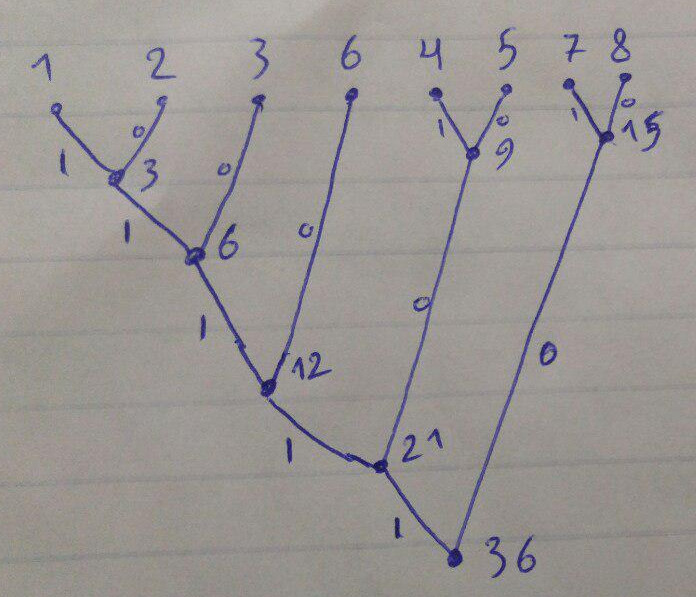
\includegraphics[width=0.50\textwidth]{1a.jpg}
 \caption{Huffman algorithm output
 \label{fig:1a}}
\end{figure}

\item (b) Suppose the alphabet $\{ a_1, a_2, a_3, a_4, a_5\}$ with 
$\{5,6,7,8,15\}$ weights. The node generated from $/{a_1, a_2/}$ is going to
merge with two possible nodes $\{a_3, a_4\}$ and $a_5$. This turns into two
possible huffman code for this alphabet.
\begin{figure}[H]
 \centering
 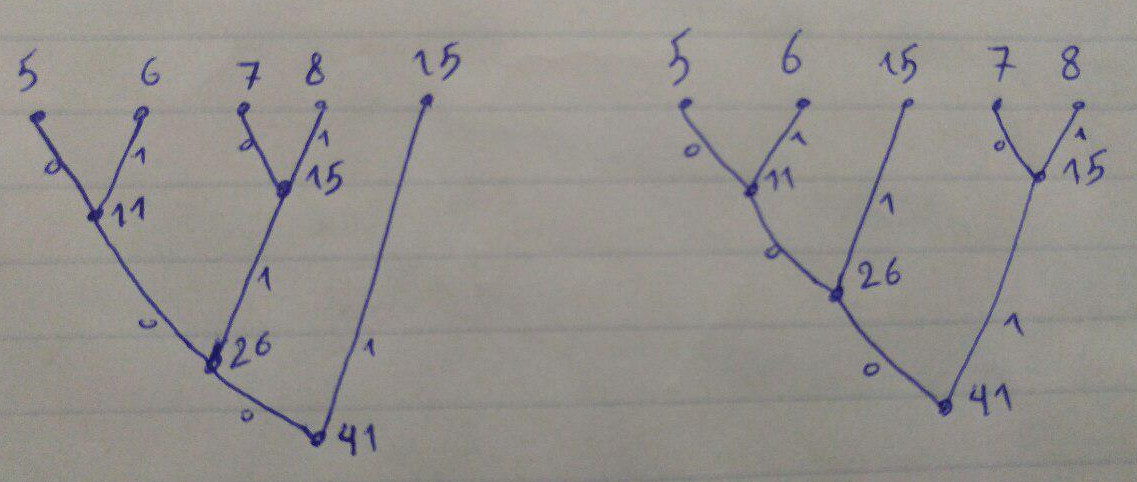
\includegraphics[width=0.50\textwidth]{1b.jpg}
 \caption{Two different Huffman codes
 \label{fig:1b}}
\end{figure}

\end{itemize}
\end{solution}


\begin{problem}{2}
A greedy algorithm for El Goog
\end{problem}

%Below is the solution environment
\begin{solution}{}
This problem has a greedy solution that we can sort the jobs by their $f_i$,
and run jobs based on their decreasing order of $f_i$.
\\
Suppose that this solution $S$ is not an optimal solution and the optimal solution
is $S^{*}$. Suppose two consecutive jobs $J_i$ and $J_j$ in $S^{*}$ that
$f_i \leq f_j$. We are going to swap these two consecutive jobs to create a new
solution $S^\prime$ and prove that this will not increase the completion time. The
starting time of the jobs before and after these two jobs will not changed
because they are going to start their execution at $p_i + p_j$ in both cases.
The starting time of running the second part of second job in $S^*$ and $S^\prime$
is $p_i + p_j$. Hence, if the job that is going to execute later has higher 
finishing time, the completion time will be higher. In $S^*$ the second job
that is going to execute has higher finishing time, and consequently, if we
swap these two consecutive jobs this parameter will not increase because
$f_i \leq f_j$.
\\
By doing this procedure until there is not two consecutive jobs that the
finishing time of the first job is lower than the second one, we have jobs
in the decreasing order of their finishing time. Hence, the greedy solution 
is optimal. I want to add that in each swap procedure, the number of inversions
in the array of finishing times will increase and swapping procedure will end.

The time complexity of this algorithm is $\theta(nlogn)$ because we just want to sort
jobs based on their finishing times.
\end{solution}


\begin{problem}{3}
MST for near-tree
\end{problem}

%Below is the solution environment
\begin{solution}{}
By the cycle property, we know that in each cycle, the heaviest edge should not appear
in any MST. As a result, if we found a cycle in the graph and remove the heaviest edge
on it for nine times, the remained graph has $n-1$ edge, and it is connected yet, and
consequently, it will be a tree. To find a cycle in this graph we can run a DFS algorithm,
and whenever we see a back edge in the DFS algorithm, it will result to a cycle, and we 
can find the heaviest edge on that easily. 

The time complexity of this algorithm is the number of DFS algorithms we run multiply to
the time complexity of running the DFS algorithm and finding the heaviest edge. The time
complexity of DFS algorithm is $O(|V| + |E|)$ and the time complexity of finding the 
heaviest edge is $O(|V|)$ because we should go through the edges in the DFS tree and
find the heaviest edge. Moreover, the number of times we should run the DFS algorithm
is nine times, and after that, the graph will not have any cycle. 

Finally, the time complexity of this algorithm is $O(|V|+|E|)$ and because $|V|,|E| \in
O(n)$, the time complexity is $O(n)$.
\end{solution}


\pagebreak

\end{document}

